\section{Dictionary ADT}
The Dictionary ADT is similar to python's dictionaries. Formally, the data for a dictionary is a set of elements $S$ where each $x \in S$ has a field $x.$key where keys are elements of some totally ordered set (often taken to be the integers). The keys in a dictionary are unique. This means that for every $x, y \in S$ we have that $x.$key $\neq$ $y.$key. The ADT defines 3 operations on this set: \texttt{Insert}, \texttt{Search} and \texttt{Delete}.
\begin{itemize}
    \item \texttt{Insert}($S, x$): Insert $x$ into $S$. If there is some $y$ in $S$ with $y.$key = $x.$key, then replace $y$ with $x$.
    \item \texttt{Search}($S, k$): Return $x$ in $S$ for which $x.$key = $k$. Return null if no such $x$ exists
    \item \texttt{Delete}($S, x$): Delete $x$ from $S$ (note they parameter is $x$, \textit{not} the key)
\end{itemize}

Quite often we think of $x$ as consisting of two parts: the key and everything that is not the key. This remaining part can be called the value of $x$, turning $x$ into the more familiar (\textit{key, value}) pairing.

There are a number of different ways of implementing this ADT, we see some examples below.

\subsection{Direct-Access Table}
Perhaps the simplest way is to create a location in memory for every possible key. For example suppose the only possible keys are numbers 0 -- 99. In this case we can create an array of size 100 and store an inserted value in the appropriate index. In this case, \texttt{Search}, \texttt{Insert} and \texttt{Delete} are all constant time. Of course what we gain in time, we lose in space (if instead the index was given by 32-bit numbers, we would need $2^{32}$ locations in memory!). So we end up reserving an enormous amount of space for ($key, value$) pairs that may never be used.

\begin{figure}
    \centering
    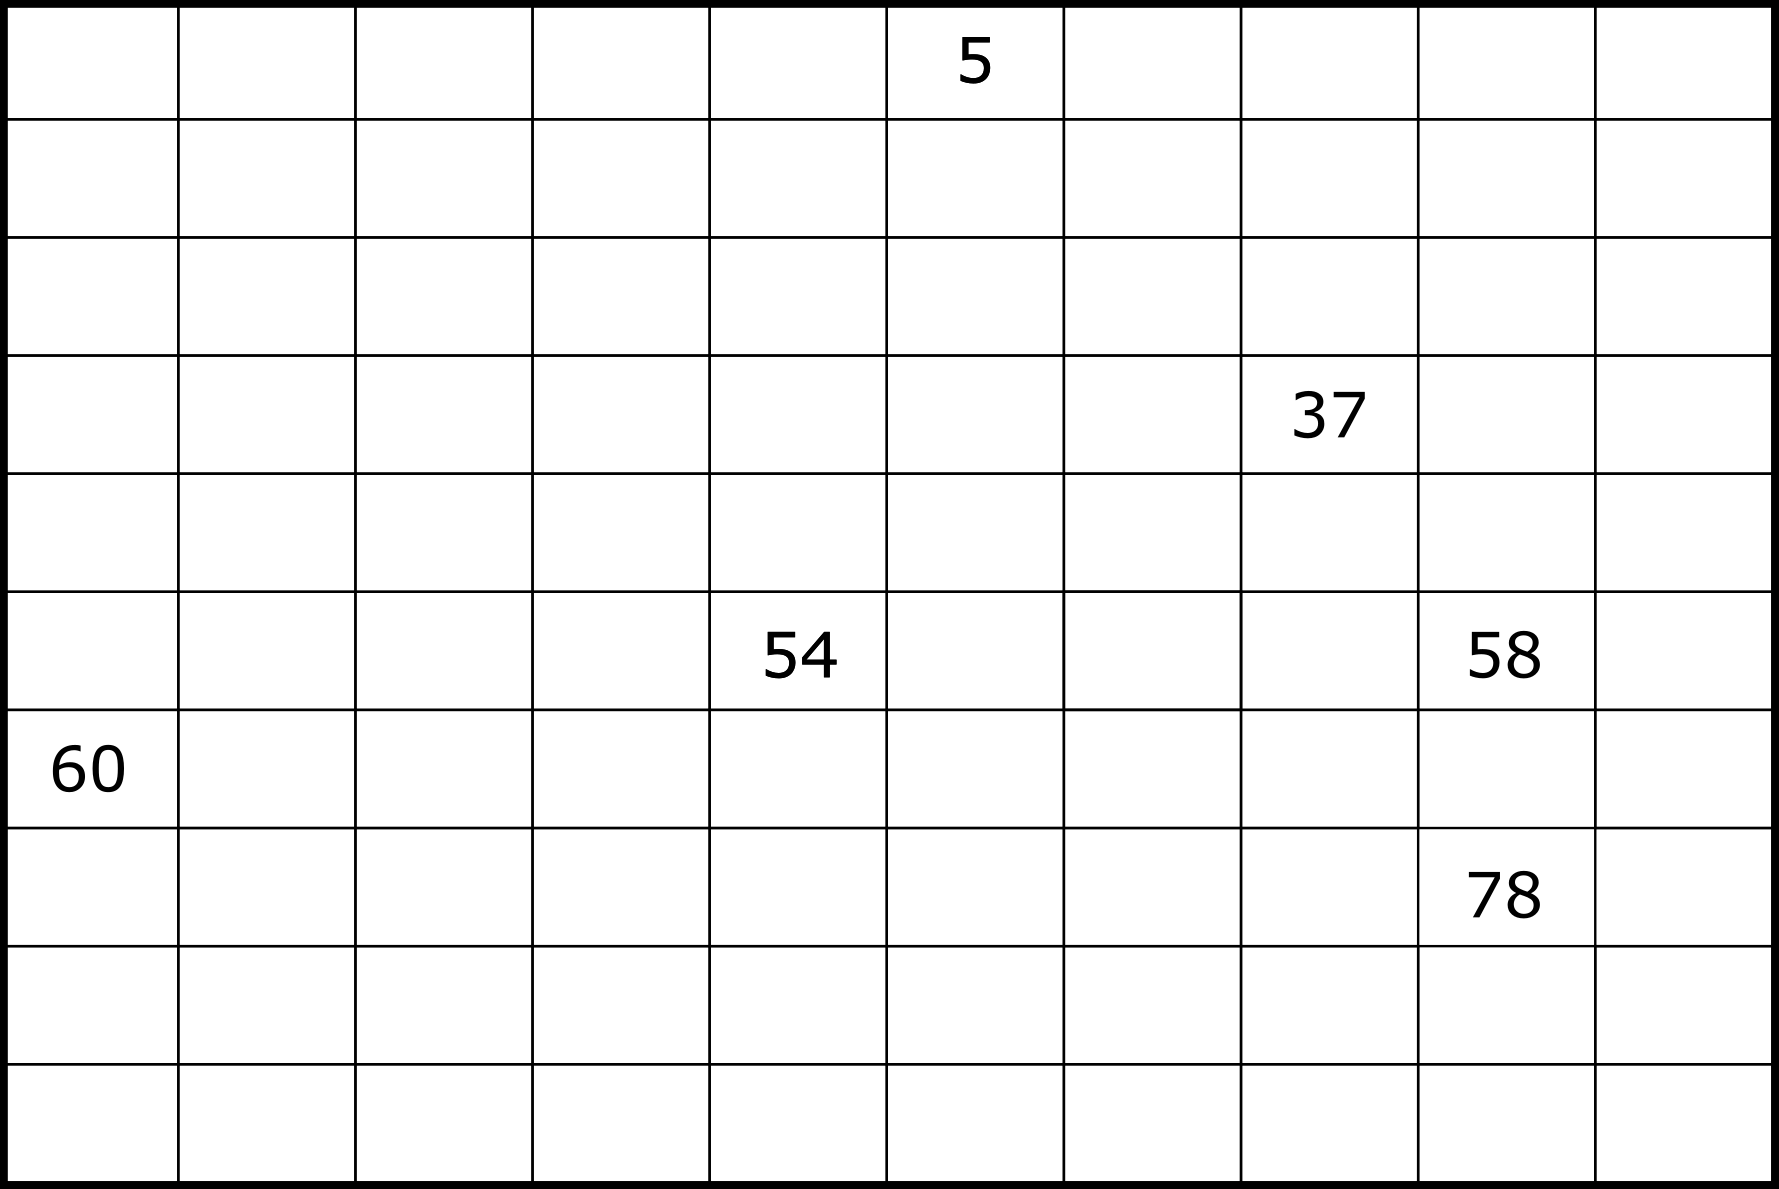
\includegraphics[scale=0.3]{Images/direct_access_table.png}
    \caption{Direct-access Table}
    \label{fig:dat}
\end{figure}

\subsection{Hash Table}
We can perhaps make things a bit easier by using a hash function. A hash function allows us to map the entire universe of possible keys to a smaller collection and we use this smaller collection to access the table. 

Of course by its very nature, there will be conflicts in this mapping -- the hash function cannot be injective. This means that we need to deal with two different keys being mapped to the same value by the hash function. We discuss this in detail in \autoref{sec:hashing} but a common way of dealing with this is storing the values corresponding to a hashed key as a linked list. In other words each entry in the direct access table for the hashed keys actually points to the head of a linked list. In this worst case, we simply have the items being stored in a linked list which (as we see below) take $\Theta(n)$ time for searching (however the average case can be made $\Theta(1)$ as we will see later, so this is certainly not a bad alternative). Insertion and deleting take $\Theta(1)$ time (assuming we have already searched for the item).

\begin{figure}[h]
    \centering
    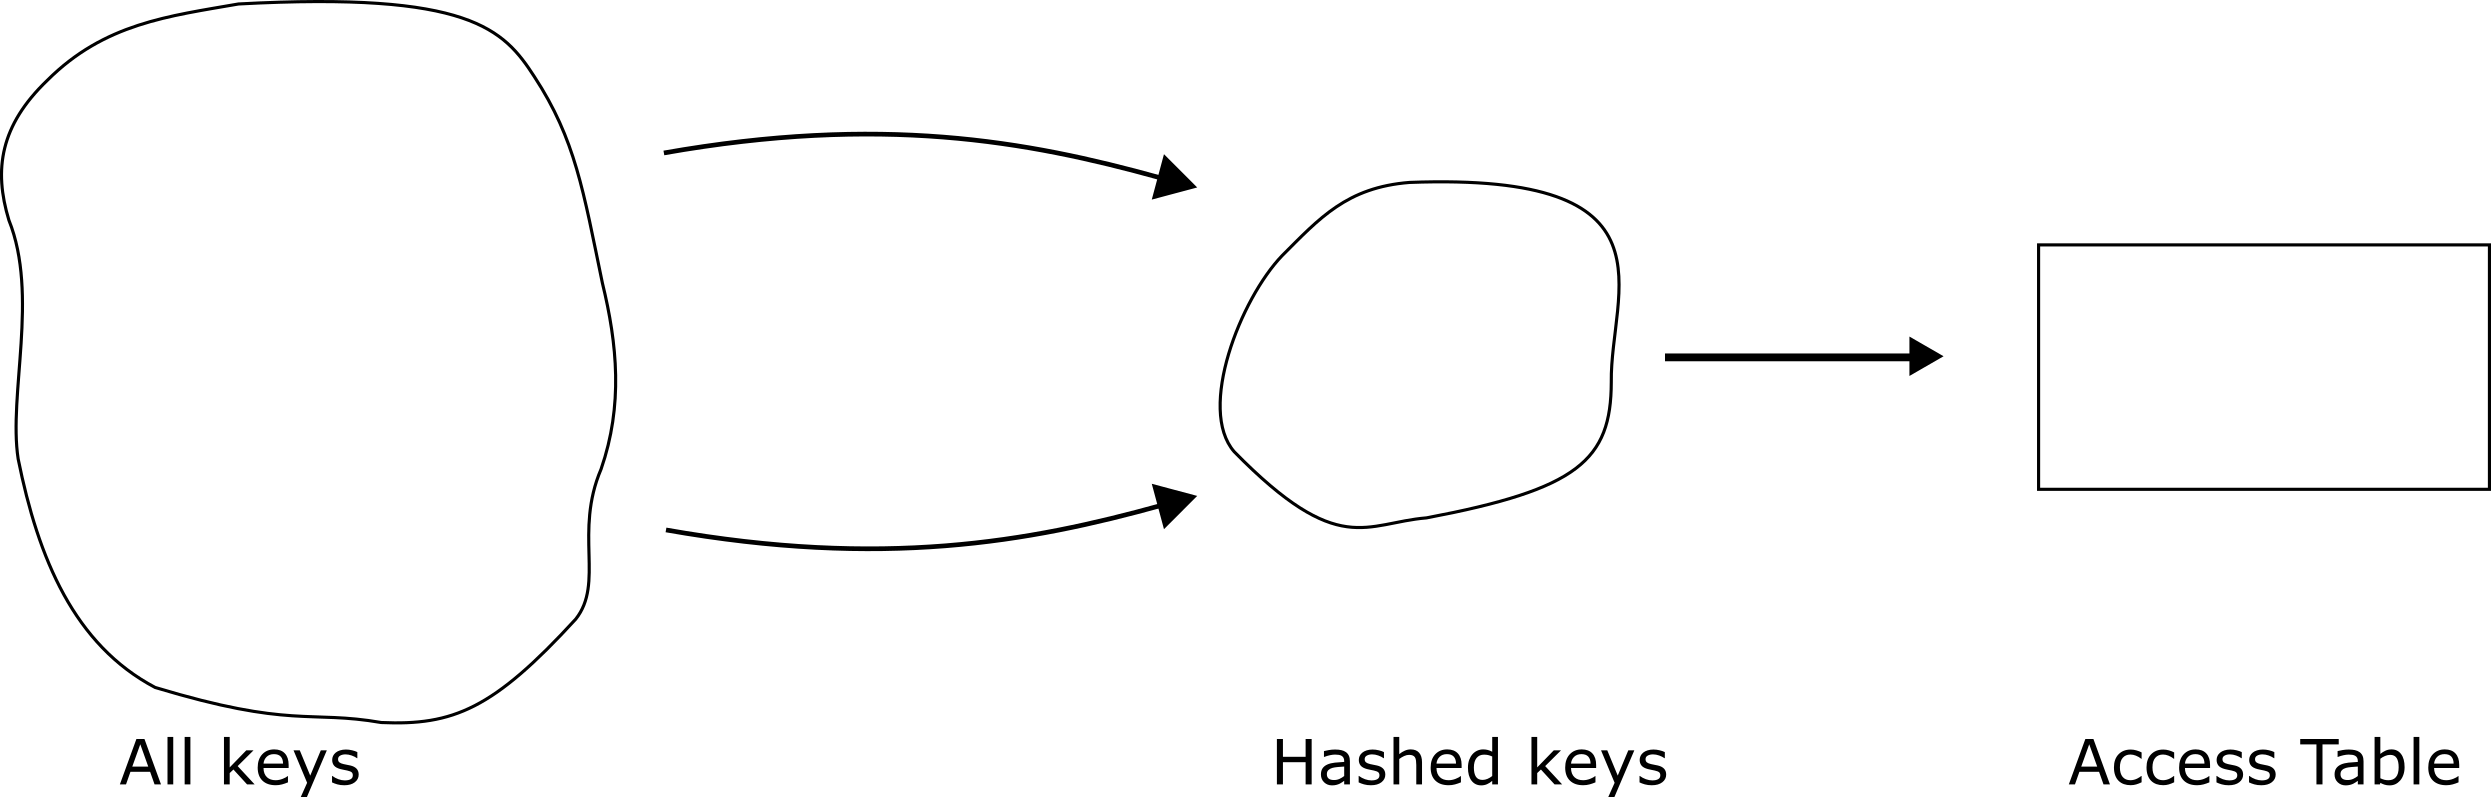
\includegraphics[scale=0.3]{Images/hash_table.png}
    \caption{Hashing keys}
    \label{fig:hash_table}
\end{figure}

\subsection{Array}
Another way we might try to remedy the situation with Direct Access tables is to simply add things to the array when needed, instead of allocating space at the beginning. In this case, when searching we need to iterate over every value in the array in order to determine whether it contains the specified key or not making this $\Theta(n)$. Insertion and deleting however are $\Theta(1)$ (assuming we keep track of the dictionary size, we simply add new items to the corresponding position and after we remove an item we can use the last item to fill the gap. Both of these operations are constant time).

In the above we assume arrays to be unsorted. If we sort the array, then searching becomes $\Theta(\log n)$ (we use binary search) but now insertion and deleting become $\Theta(n)$ since we need to shift items in order to preserve the ordering.

\subsection{Linked List}
With an unsorted linked list the situation is much the same as before, searching is $\Theta(n)$ while insertion and deleting are quite cheap, being constant time (as always, we assume the insertion and deletion happen \textit{after} a search is performed, so we don't account for the time spent on searching). The situation remains exactly the same if we sort the linked list instead since we cannot access the central element of the list in order to perform binary search.

\subsection{Binary Search Tree}
The above seems to very strongly suggest using a binary search tree since we point directly to the central element! Unfortunately in the worst case a binary search tree could be completely one-sided an simply be a linked list. If only there were some way of ensuring that a binary tree were balanced...

\subsection{Balanced Search Trees}
This is of course what inspires the category of what are called balanced search trees that try to minimise the height of a tree as much as possible. There are many different kinds such as red-black trees, AVL trees, B trees, etc. We will look at AVL trees.

\section{Binary (Search) Trees}
We take a brief refresher with binary trees before delving into how to balance them.

A binary tree is simply a tree where each node has at most 2 children. As usual, if a node has no child it is called a leaf. The height of a tree is the size of the longest path between the root and its leaves (where the size of the path is given by the number of edges traversed, in particular then a single node tree is of height 0). The depth of a node is the size of the path from the root to that node. We can then equivalently define the height of the tree as the maximum depth of any node in the tree.

A binary tree is called a binary search tree if every node satisfies the binary search tree property: everything on the left subtree of a node is smaller than or equal to the node and everything on the right is greater than or equal to the node.


\begin{figure}[h]
    \centering
    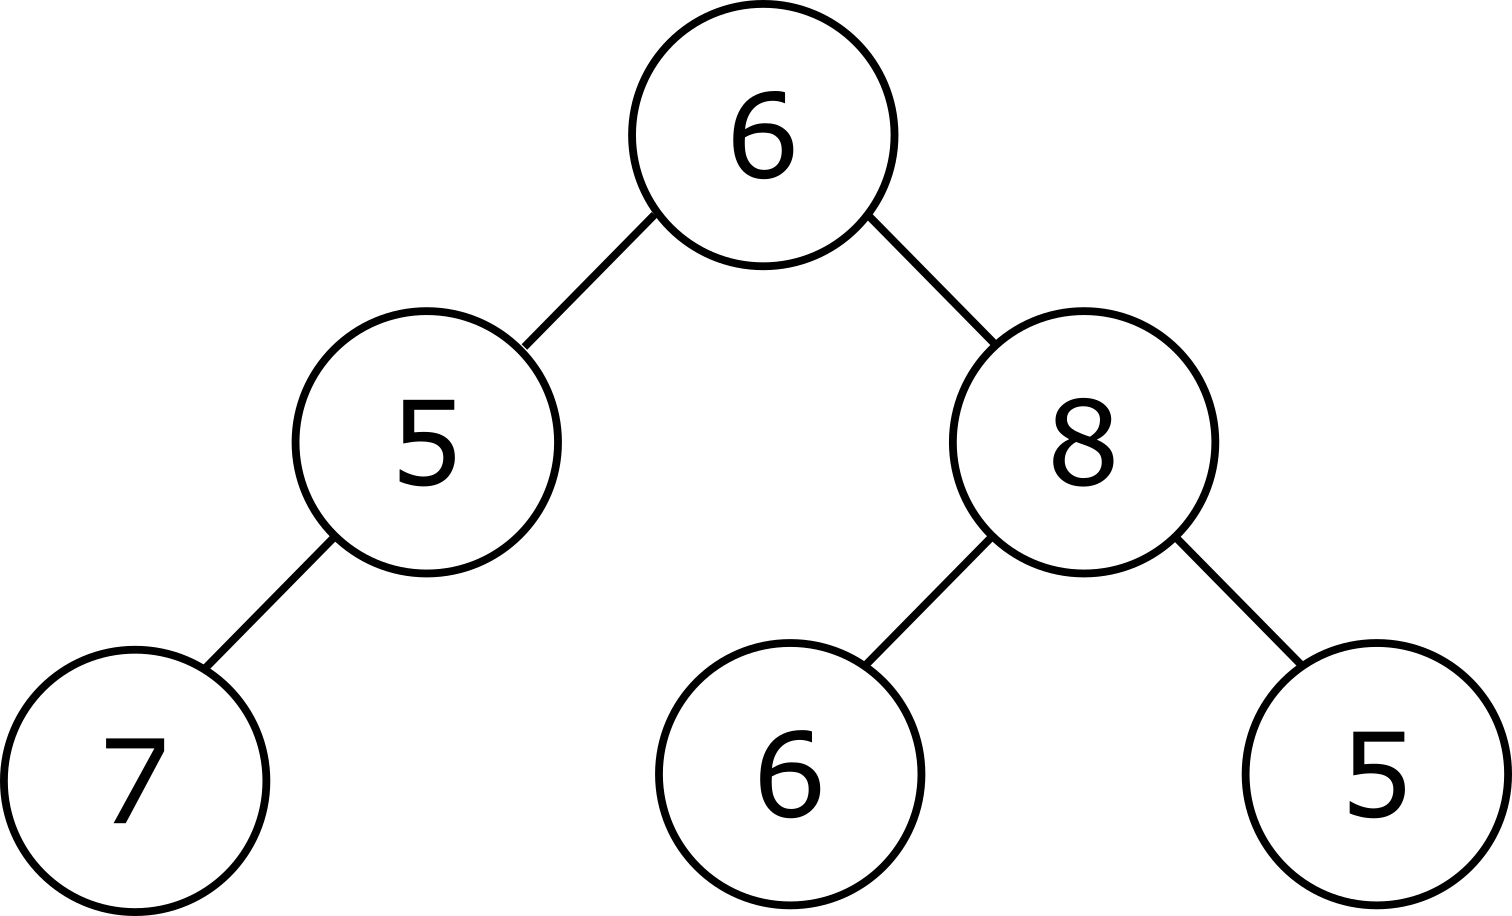
\includegraphics[scale=0.3]{Images/non_bst.png}
    \caption{Example of non-BST}
    \label{fig:non_bst}
\end{figure}
\begin{figure}[h]
    \centering
    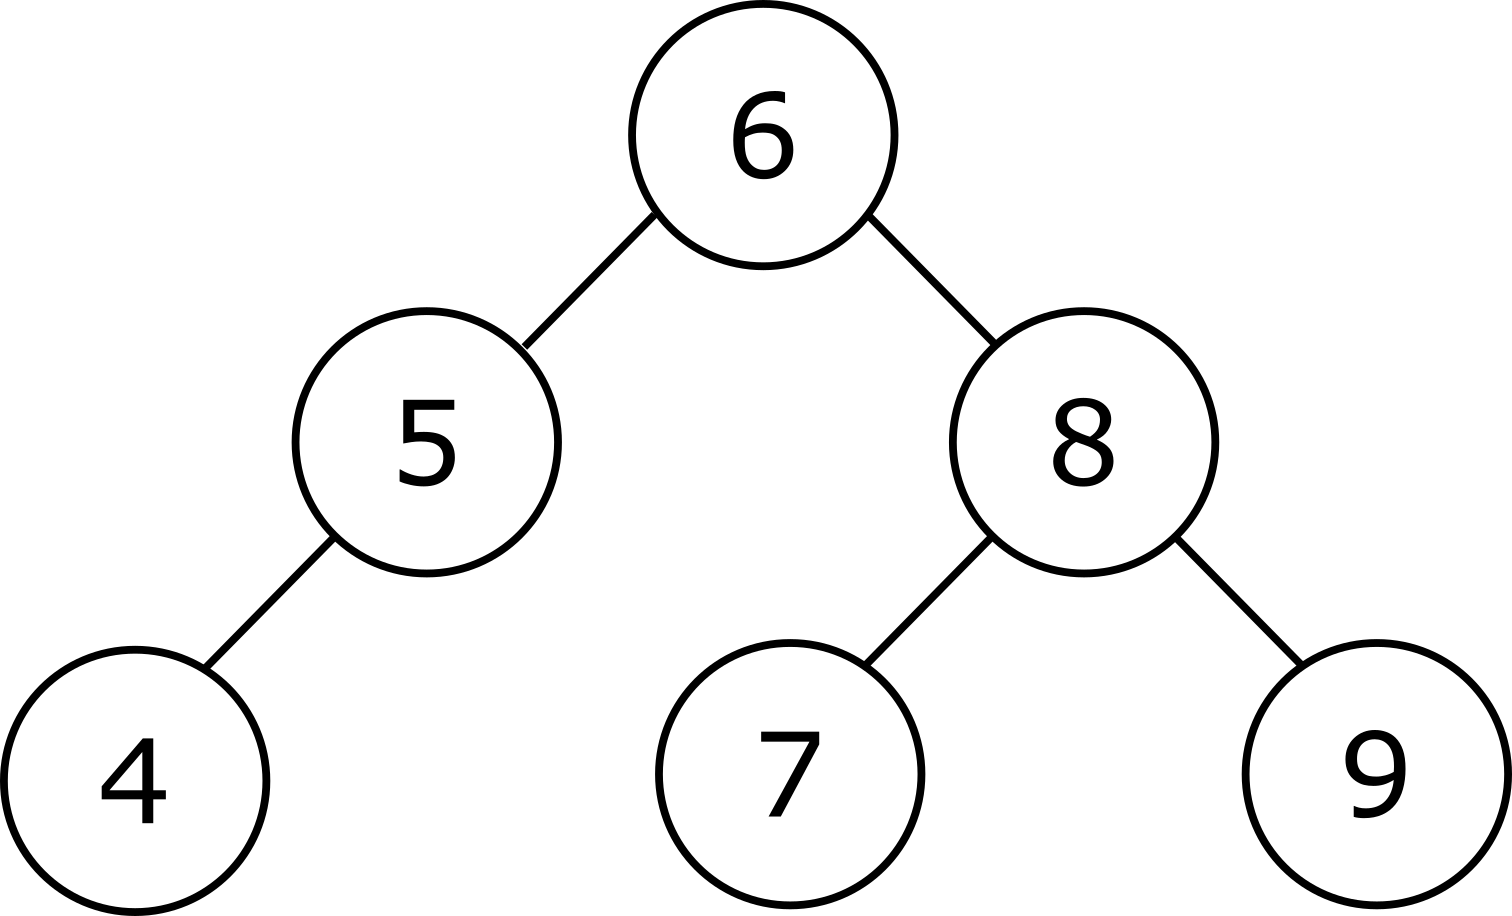
\includegraphics[scale=0.3]{Images/bst_example.png}
    \caption{Example of BST}
    \label{fig:bst_example}
\end{figure}

\subsection{Insert}
Now we consider how we might implement the Dictionary ADT using a binary search tree. First we recall that the keys of a dictionary are unique, so we know that everything on the left subtree is going to strictly smaller than the root which in turn is going to strictly smaller than everything on the right subtree. The insertion algorithm for a BST might look something like so\\
\begin{lstlisting}[language=Python]
INSERT(S, x):
    # Helper may need to modify the root itself: have it return value.
    S.root <- TREE-INSERT(S.root, X)
    
TREE-INSERT(root, x):
    if root is NIL: # x.key not already in S
        # Found insertion point: create new node with empty children
        root <- TreeNode(x)
    else if x.key < root.item.key:
        root.left <- TREE-INSERT(root.left, x)
    else if x.key > root.item.key:
        root.right <- TREE-INSERT(root.right, x)
    else: # x.key == root.item.key
        root.item <- x # replace root with x
    return root
\end{lstlisting}
\begin{remark}
    Note that $S$ doesn't technically store the whole tree. It only stores (a pointer to) the root and we can recursively go through the tree using \ttt{.left} and \ttt{.right}.
\end{remark}

It is then clear that the runtime for \ttt{Insert} depends on the the height of the tree. Also note that the same set of numbers could give us completely different trees, depending on the order in which they are inserted (see \autoref{fig:rough_balanced_bst}). We will see that this is a primary concern with binary trees.

\begin{figure}[h]
    \centering
    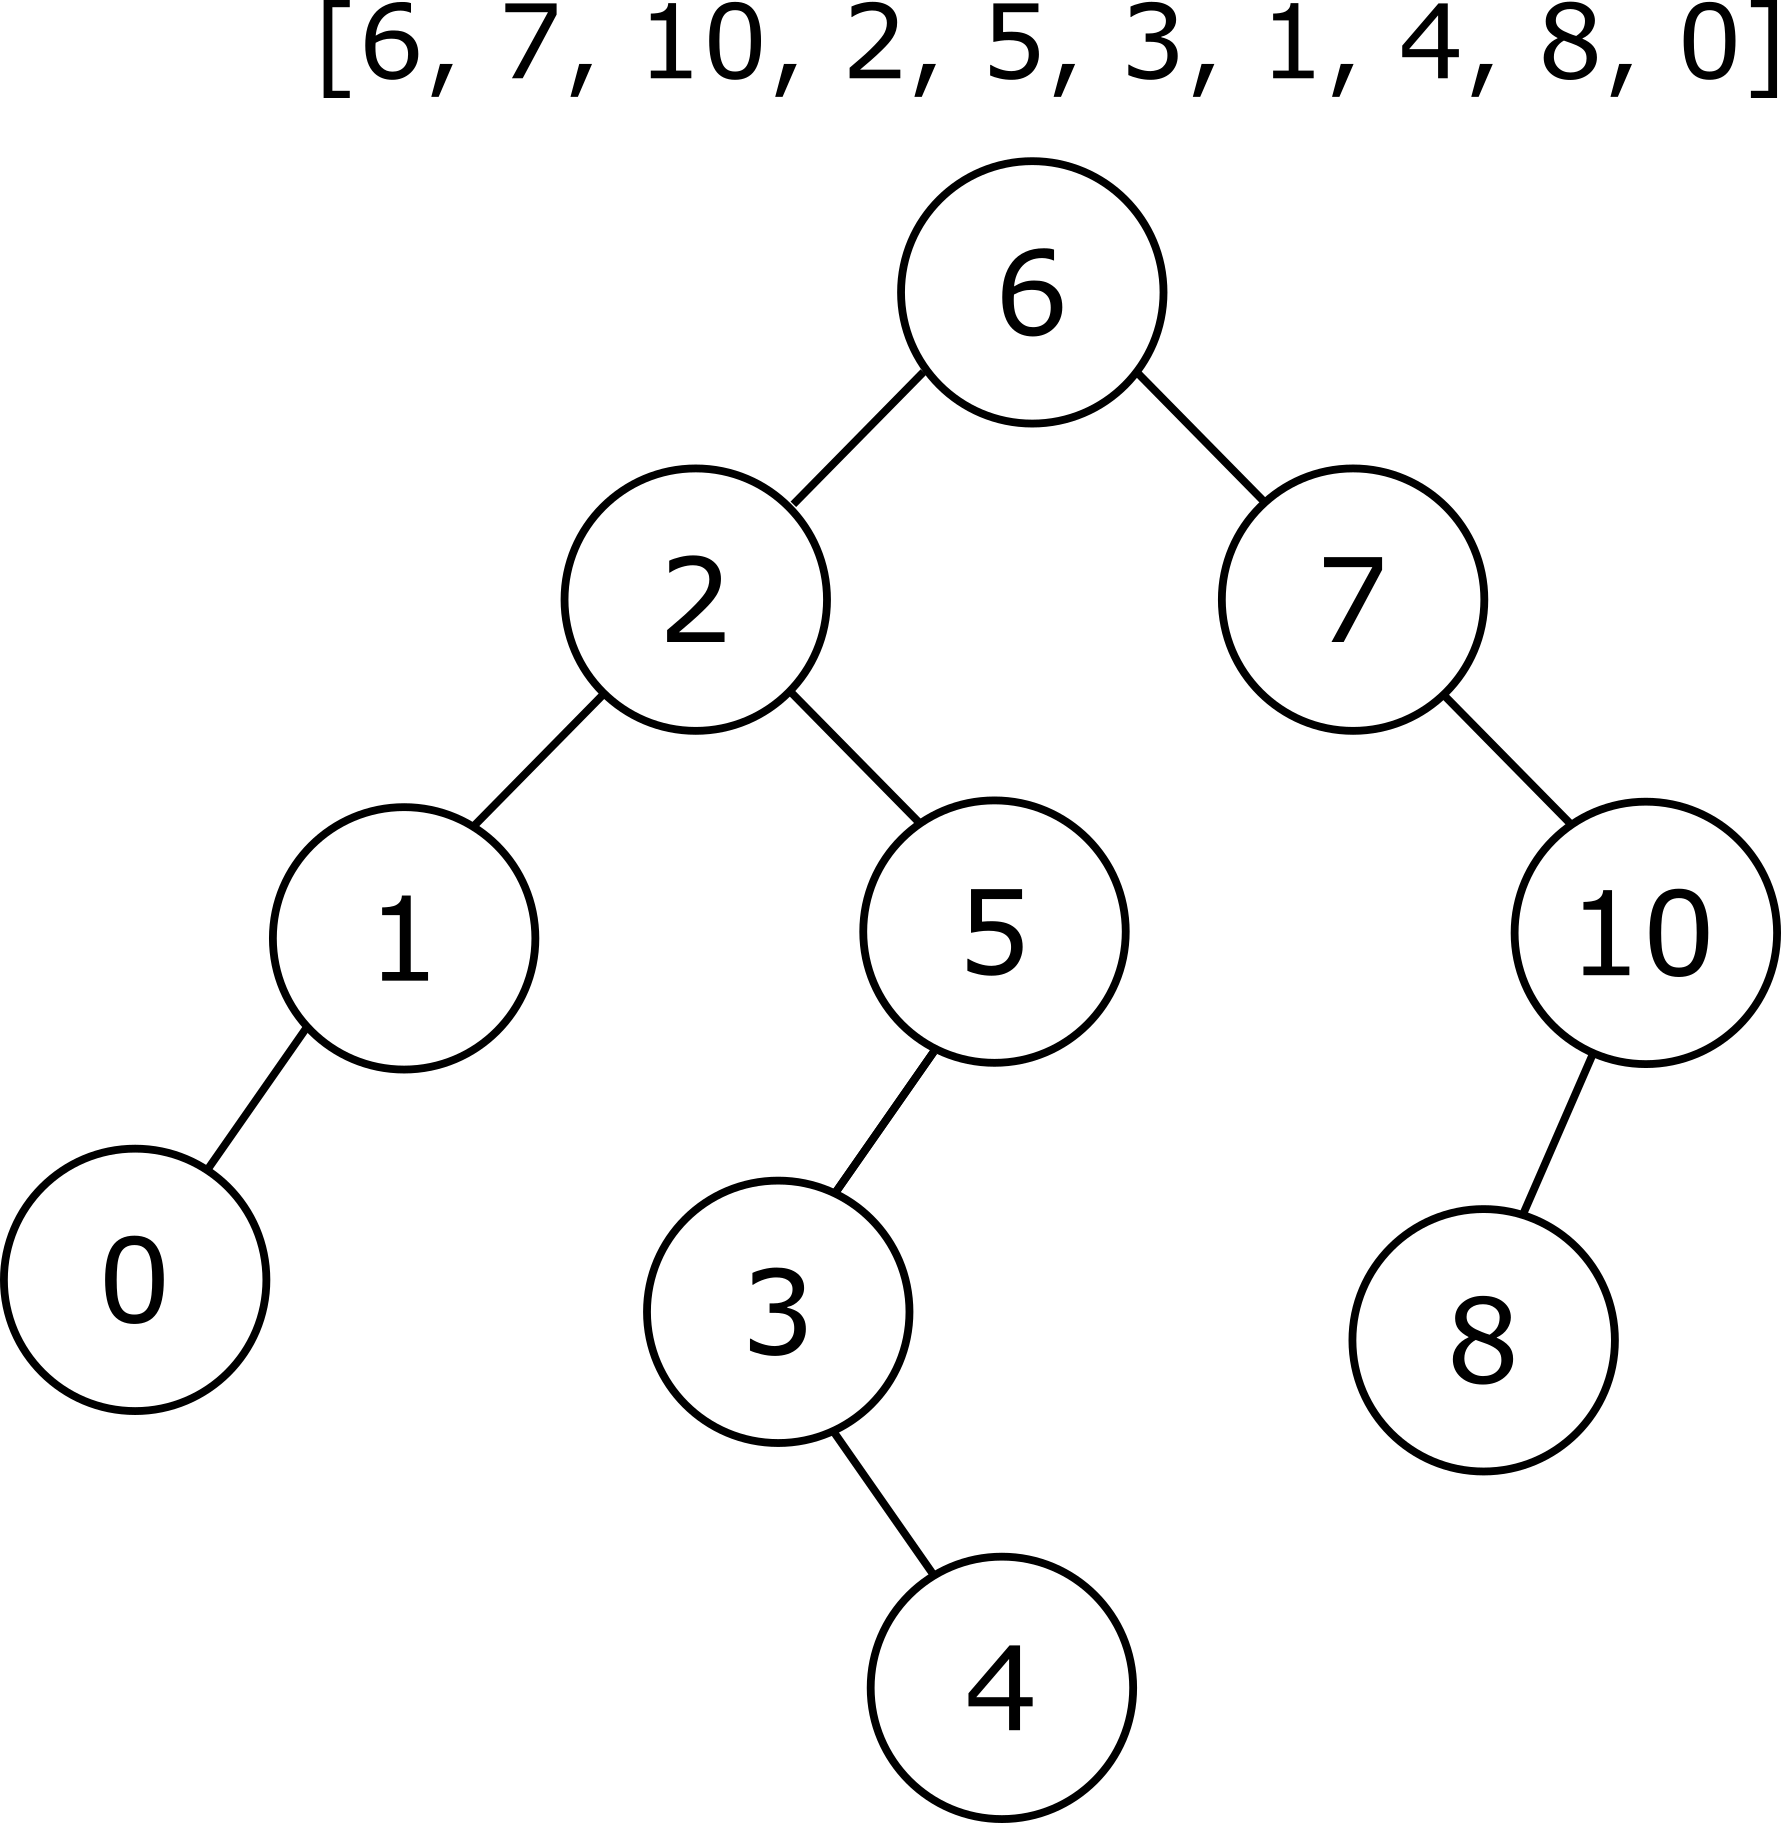
\includegraphics[scale=0.15]{Images/insertorder1.png}
    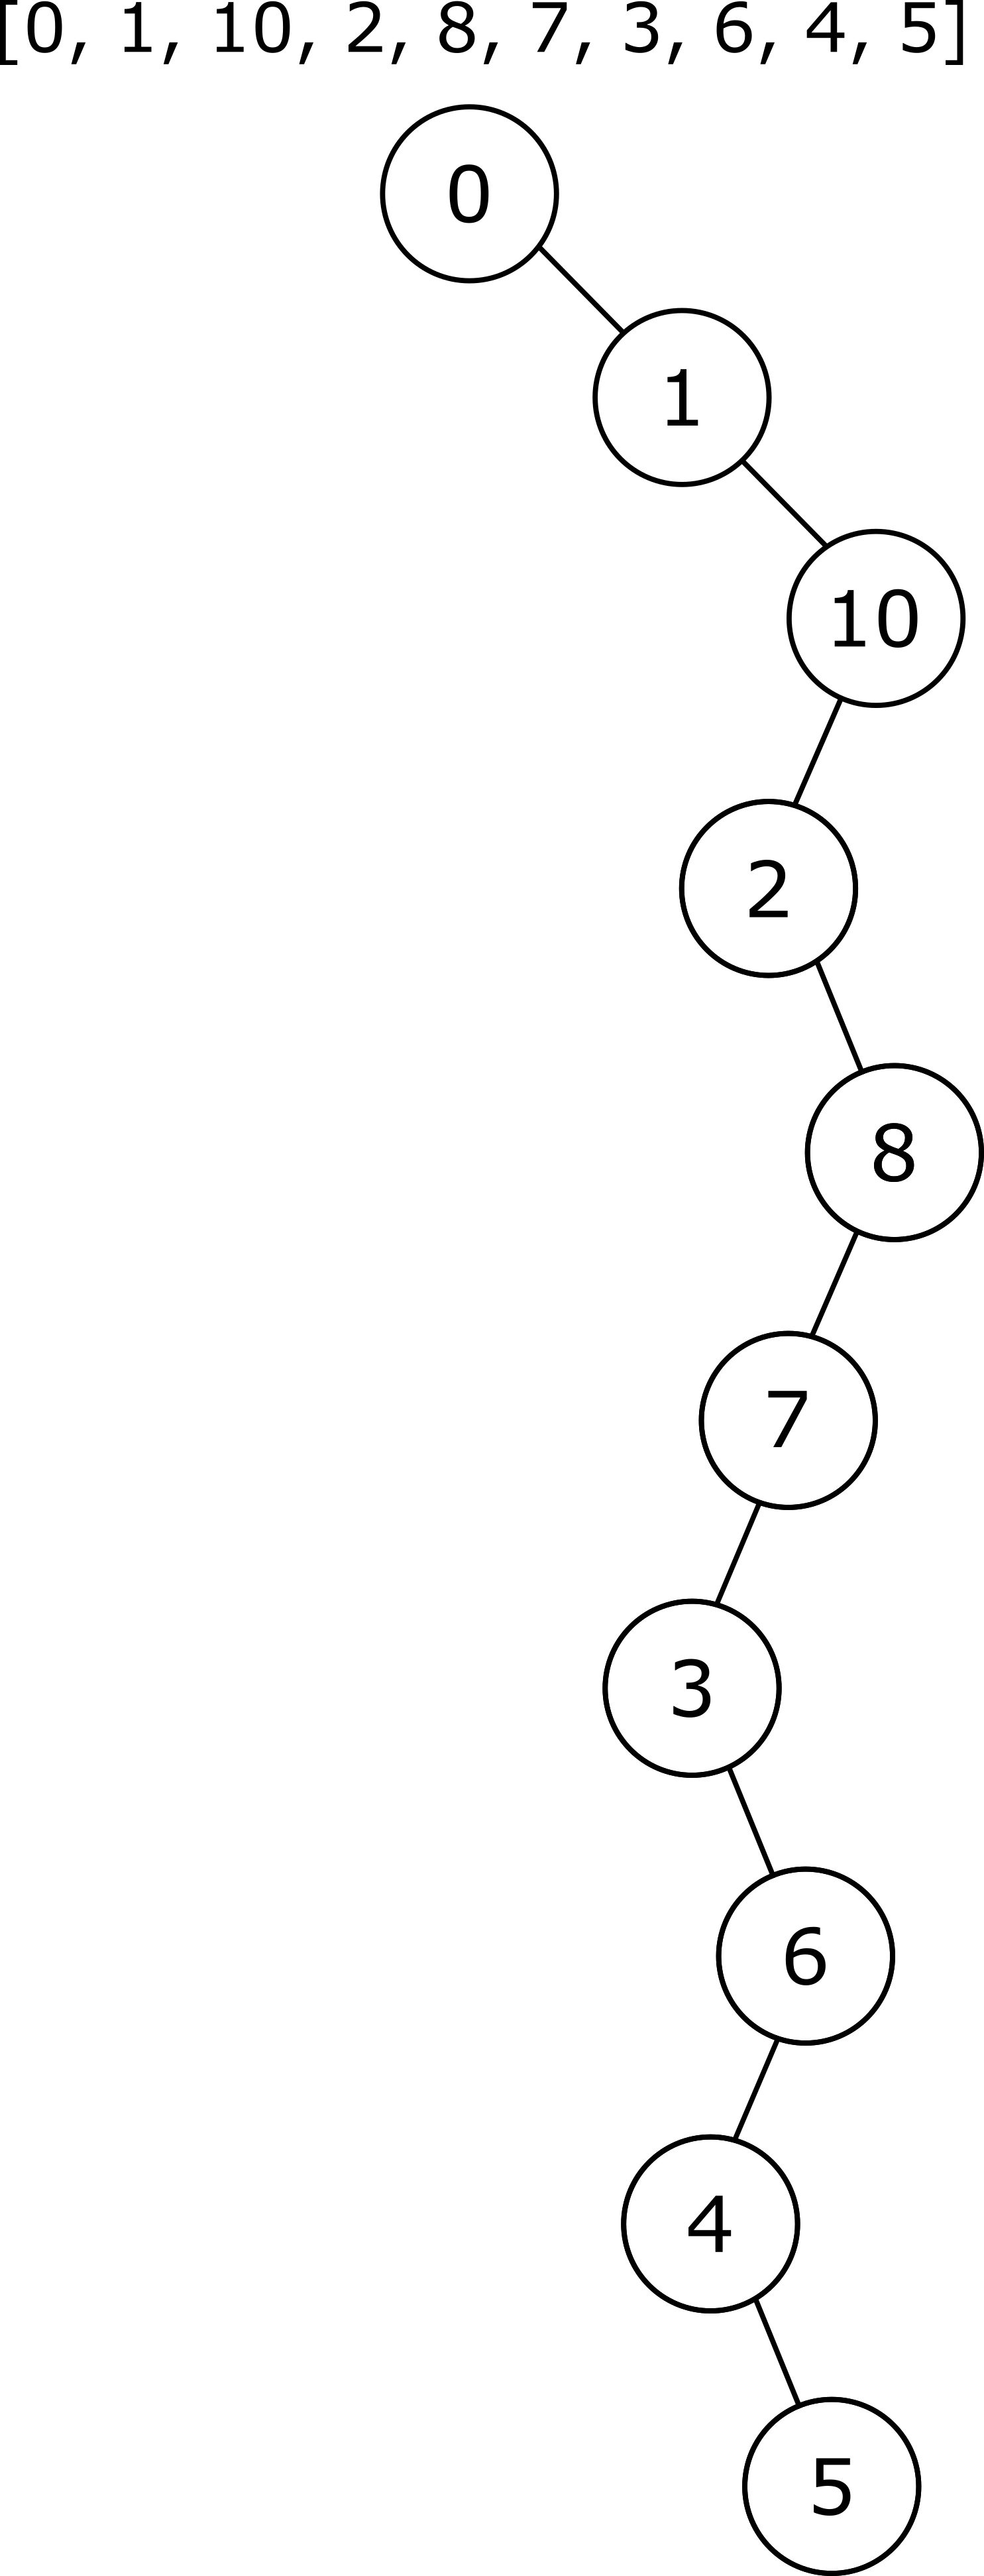
\includegraphics[scale=0.15]{Images/insertorder2.png}
    \caption{Dependence of BST on insertion order}
    \label{fig:rough_balanced_bst}
\end{figure}

\subsection{Search}
An algorithm for \ttt{Search} can be described like so
\begin{lstlisting}
SEARCH(S, k):
    return TREE-SEARCH(S.root, k)
    
TREE-SEARCH(root, k):
    # Compare root.key with k to determine if k is to the left or right
    # return when root.key == k
    if root is NIL: # k not in S
        pass
    else if k < root.key:
        root <- TREE-SEARCH(root.left, k)
    else if k > root.key:
        root <- TREE-SEARCH(root.right, k)
    else: # we have found the key
        # root.key == k
        pass
    return root
\end{lstlisting}

Once again the runtime is dependent on the height of the tree, which in the worst case is simply the number of items.


For illustrative purposes, we can analyse the expected number of calls to search among the two trees above in \autoref{fig:rough_balanced_bst}, assuming that $k$ is chosen uniformly from $\{0, \dots, 10\} \backslash \{9\}$. We note that there are $d + 1$ calls to \ttt{TREE-SEARCH} to find a node a depth $d$. The probability of choosing any node is simply $\frac{1}{10}$. Thus for the first binary tree, the expected number of calls is
\begin{align*}
    E(T_1) = &\sum_{n} P(k = n)(\text{number of \ttt{TREE-SEARCH} calls to find node }n)\\
    &=\frac{1}{10}(1 \cdot 1 + 2 \cdot 2 + 3 \cdot 3 + 4 \cdot 3 + 5 \cdot 1) = 3.1
\end{align*}

For the second binary tree, as every node is at a different depth, we simply have
\begin{align*}
    E(T_2) &= \sum_{k = 1}^{10} \frac{1}{10} \cdot k\\
    &= \frac{1}{10} \cdot \frac{10 \cdot 11}{2}\\
    &= 5.5
\end{align*}
As one would expect, the taller tree on the right will require more function calls on average.

\subsection{Delete}
There are three distinct cases to consider when deleting from a BST. The easiest case is when we are asked to delete a leaf-- we simply delete. If the node has only one child, then the task is also quite straightforward, we promote the sole child to the place of the deleted node. The difficult case is when deleting a node that has two children. In this case, we can replace the node we want to delete with the predecessor (the rightmost node on the left subtree) or the successor (the leftmost node on the right subtree).
\begin{remark}
    In this course, we \textbf{always} replace the deleted node with the successor.
\end{remark}

We have the following algorithm for this
\begin{lstlisting}
TREE-DELETE(root, x):
    if root is NIL: # x.key not in S, should not happen
        pass
    else if x.key < root.item.key:
        root.left = TREE-DELETE(root.left, x)
    else if x.key > root.item.key:
        root.right = TREE-DELETE(root.right, x)
    else: # x.key == root.item.key so we remove root.item
        if root.left is NIL:
            root = root.right # NIL if both children missing
        else if root.right is NIL:
            root = root.left
        else:
            # Means root has two children
            # Want to remove min item in right subtree
            # Assumption: DELETE-MIN returns two values:
            # - element removed from right subtree
            # - root of resulting subtree
            root.item, root.right = DELETE-MIN(root.right)
            
DELETE-MIN(root):
    # Remove element with smallest key in root's subtree
    # return element that was removed and root of resulting subtree
    if root.left is NIL:
        # Root stores item with smallest key; replace with right child.
        return root.item, root.right
    else:
        # Left subtree not empty; root not the smallest
        item, root.left = DELETE-MIN(root.left)
        return item, root
\end{lstlisting}

As usual the runtime of this is dependent on the height of the tree which we can minimise by balancing the tree.

\subsection{Duplicate Keys}
We take a brief segue to discussing the problem of how one may implement a Dictionary ADT that allows for duplicate keys to occur using a BST. There are various strategies for how one may deal with duplicate values. In this case we will analyse the different strategies by considering what happens in the case when we try to insert $n$ identical items. 

The simplest strategy we could have for handling duplicate keys is to always put duplicates in the right subtree. We can easily modify the code for \ttt{TREE-INSERT} in order to achieve this.

\begin{lstlisting}
INSERT(S, x):
    # Helper may need to modify the root itself: have it return value.
    S.root <- TREE-INSERT(S.root, X)
    
TREE-INSERT(root, x):
    if root is NIL: # x.key not already in S
        # Found insertion point: create new node with empty children
        root <- TreeNode(x)
    else if x.key < root.item.key:
        root.left <- TREE-INSERT(root.left, x)
    else:
        root.right <- TREE-INSERT(root.right, x)
    return root
\end{lstlisting}

Now we consider our test case of inserting $n$ duplicates into an empty tree and ask how much time this takes. Assume that one call to \ttt{TREE-INSERT} takes time $c$. At depth $k$, we need to make $k + 1$ calls to \ttt{TREE-INSERT}. Therefore the time taken to insert $n$ duplicate items is
\begin{align*}
    \sum_{k = 1}^{n} k = \frac{n(n + 1)}{2}
\end{align*}
Thus the operation is $\Theta(n^2)$ for this case.

An alternative we might consider is to alternate going left and right. In particular, we add a boolean flag to each node, which dictates whether duplicates should go to the left or the right. Then each time a duplicate is inserted, the flag is inverted so that the next duplicate will be inserted in the opposite direction.

% TODO: Add diagram for boolean flag method

Let us try our test case again. We see that the height of the final tree (after all $n$ items are inserted) is $\log n$. In fact if the tree has $m$ items at a stage it will take $\Theta(\log m)$ time to insert another item. Therefore the total time taken is
\begin{align*}
    \sum_{m = 1}^{n} c \log m = c \sum_{m = 1}^{n} \log m < c \sum_{m = 1}^{n} \log n = c n \log n
\end{align*}
Hence the insertion is now $O(n \log n)$, a considerable improvement! Let us show that we are in fact in $\Theta(n \log n)$.
\begin{align*}
    \sum_{m = 1}^{n} c \log m > \sum_{m = \frac{n}{2}}^{n}c \log m > c \sum_{m = \frac{n}{2}}^{n} \log \left(\frac{n}{2}\right) = c \frac{n}{2} \log \left( \frac{n}{2} \right) = \frac{c}{2}(n \log n - 1)
\end{align*}
\begin{remark}
    Note the `trick' above of only considering half the sum. This is a useful technique for finding lower bounds.
\end{remark}
Thus with this approach we are in $\Omega(n \log n)$ as well implying that we are indeed taking $\Theta(n \log n)$ time.